\subsection{Standard Signals}
To validate the iPad application, the prototype was tested with standard signals. The voltage applied to each input pin is summarised in Table~\ref{table: standard signals}. The A0 pin on the Arduino, corresponding to glucose, was tested with a random noise signal. The A1 pin, corresponding to lactate, was tested with a square wave. The A7 pin, corresponding to potassium, was tested with a sine wave. 

\begin{table}[h!]
\centering
\begin{tabular}{||c c c||} 
 \hline
 Input Pin & Electrochemical & Signal Description \\ [0.5ex] 
 \hline\hline
 A0 & Glucose & Noise signal, 1V P-P voltage, 0.5V offset \\
 A1 & Lactate & 0.1Hz square wave, 1V P-P voltage, 0.5V offset \\
 A7 & Potassium & 0.1Hz sine wave, 0.5V P-P voltage, 0.5V offset \\
 \hline
\end{tabular}
\caption{Standard signals received by input pins.}
\label{table: standard signals}
\end{table}

The signals were chosen to have a low frequency of 0.1Hz since the electrochemical signals present during the occurrence of an SD display changes slowly and over a long time frame. Furthermore, the app only receives data once every second from each input, hence according the the Nyquist rate, frequencies above 0.5Hz will undergo aliasing and will not be reconstructed well.

The standard signals inputted to the Arduino pins were produced by a signal generator. In parallel, these signals also went to a PicoScope input channel, which was then connected to a laptop so that the signals could be recorded on PicoLog with a sampling frequency of 5Hz. The signals displayed on PicoLog could then be compared with the signals received on the iPad app post processing and transmission. Figure~\ref{fig: test1} shows the setup of the experiment.

\begin{figure}[h!]
\centering
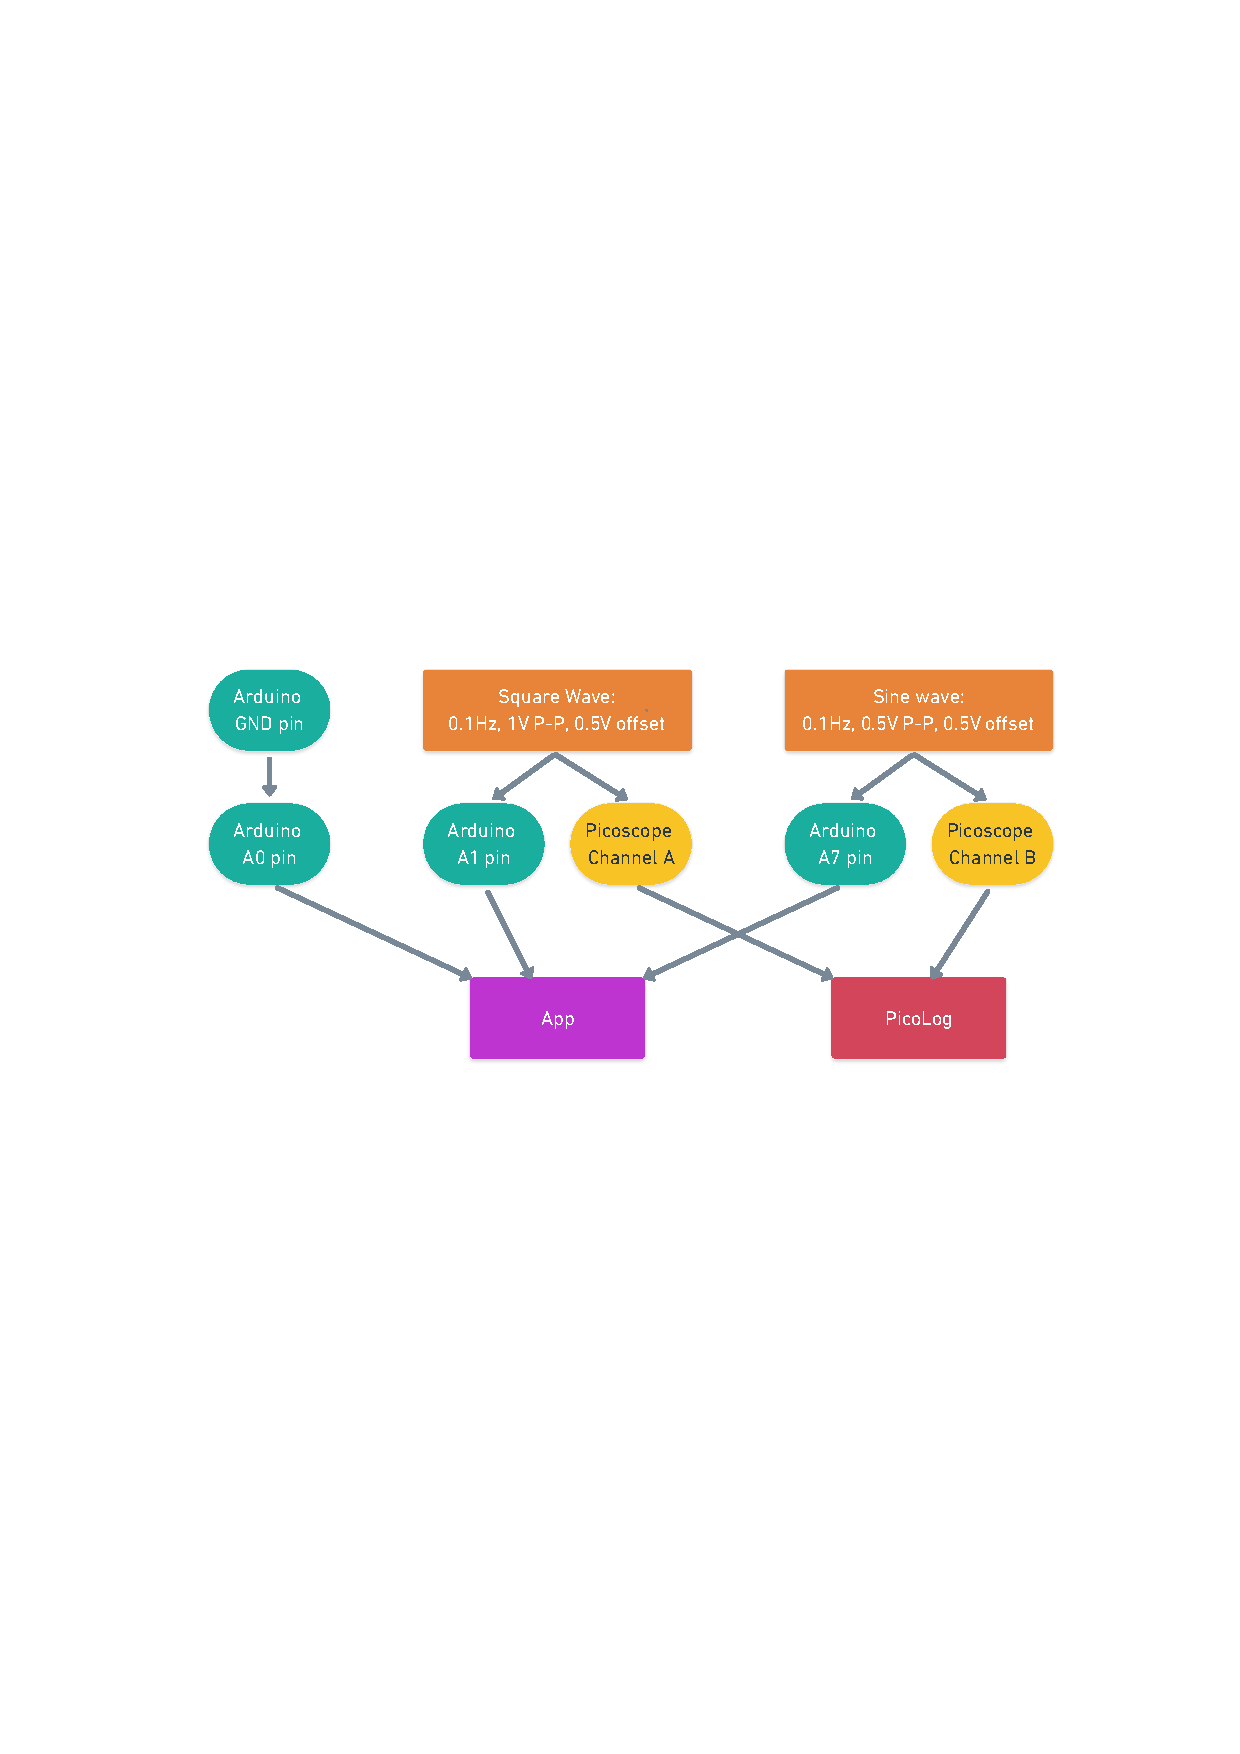
\includegraphics[trim={0cm 3.5cm 0cm  3.5cm}, clip, width=1\textwidth]{./figures/test1.pdf}
\captionsetup{justification=centering}
\caption{Experimental setup for testing standard signals.}
\label{fig: test1}
\end{figure}


\subsection{Spreading Depolarisation}
This test aimed to see if the characteristics of the SD could be visualised on the app. From previous research \cite{Rogers2017}, 18 minutes of potassium, glucose, and lactate patient data, which included the occurrence of an SD, was obtained. The signals were downsampled from 200Hz to 50Hz to reduce the signal lengths to less that 60,000 samples so that it could be programmed onto the arbitrary waveform generator (AWG). No significant information was lost in the downsampling process as the frequency spectrum of the extracted signals showed high power for frequencies less than 1Hz. The characteristics of the extracted electrochemical signals are shown in Table~\ref{table: patient data}. 


\begin{table}[h!]
\centering
\begin{tabular}{||c c c c c||} 
 \hline
 Electrochemical & P-P Voltage & SD range & Amplification & Capping\\ [0.5ex] 
 \hline\hline
 Glucose & -4.29V -- 6.8V & 0.35V -- 0.7V & No & Yes \\
 Lactate & 0V -- 1.903V & 0V -- 1.903V & No & No \\
 Potassium & 21.59mV -- 79.59mV & 0mV - 20mV & x100 & Yes \\
 \hline
\end{tabular}
\caption{Patient data characteristics and whether signals were amplified or capped.}
\label{table: patient data}
\end{table}

Since potassium has a low voltage range during an SD and the Arduino is limited to 4.88mV resolution, the signal was multiplied by 100 for testing purposes so that the Arduino could detect the signal with higher precision. The app was temporarily modified to divide the received signal by 100. Potassium and glucose were then processed so that the signals were capped between 0V and 5V, which is the range the Arduino can detect. The signals were then programmed into the AWG. 

Each electrochemical signal was tested one at a time since the AWG is limited to outputting one signal, and only one AWG was accessible. The output channel of the AWG was connected to an Arduino input pin depending on which signal was being tested. The other two input channels were connected to ground. Each signal was recorded on the app and then compared to the original patient data.

\begin{table}[h!]
\centering
\begin{tabular}{||c c c||} 
 \hline
 Electrochemical & Concentration (mM) & Voltage (mV) \\ [0.5ex]
 \hline\hline
 Glucose & 0.00 & 167.00 \\
  & 1.00 & 969.60 \\
  & 2.00 & 1772.20 \\
 Lactate & 0.00 & 48.77 \\
  & 0.50 & 329.12 \\
  & 1.00 & 609.47 \\
 Potassium & 2.70 & 6.05 \\
  & 6.35 & 26.27 \\
  & 10.00 & 37.00 \\
 \hline
\end{tabular}
\caption{Calibration values obtained from patient data.}
\label{table: test2 calibration}
\end{table}


As real patient data was used, it was possible to test the segmented control switch feature on the app that allows for viewing of the plots as concentration against time. Calibration values were obtained from the patient data \cite{Rogers2017} and are shown in Table~\ref{table: test2 calibration}. These values were inserted into the text fields on the app during testing.

